\chapter{Návrh a implementácia}
\label{kap:implementacia}

V kapitole opisujeme priebeh vzniku aplikácie, implementačné detaily, postupy a rozhodnutia. Základné členenie obsahu je podľa modulov, za ktoré považujeme celky aplikácie ako editor kódu v grafickom jazyku, modul pre sériovú komunikáciu či modul pre simuláciu. V rámci jednotlivých častí je opísaný ich vývoj pokiaľ možno chronologicky. Súčasťou sú tiež implementačne zmeny v riadiacich programoch robotov.

Vývoj začíname návrhom kostry a vizuálnej podoby aplikácie, v ktorej neskôr vzniknú jednotlivé moduly. V prvej fáze implementujeme časti podporujúce komunikáciu s aktuálnou verziou riadiaceho programu robota Otto a jeho programovanie. Nasleduje etapa rozširovania funkcionalít (hlavne grafického jazyka)  a práca na module simulácie.


% GUI
\section{Grafické rozhranie}
GUI aplikácie tvoríme pomocou JavaFX. Cieľom je vytvoriť prehľadné prostredie, v ktorom sa ľahko zorientuje i požívateľ nižšieho veku. Pri rozmiestňovaní jednotlivých prvkov sú nám nápomocné existujúce aplikácie, no zohľadňujeme i rady autorov knižnice Blockly \cite{blocklyBestPractices}, keďže komponent umožňujúci prostredníctvom nej programovať robota je v našej aplikácii dominantným. Z odporúčaní je zrejmé, že plochu pre manipuláciu s prvkami grafického jazyka je žiaduce maximalizovať a neoddeľovať ju od komponentu umožňujúceho tvorbu blokov (prvkov jazyka).

Ďalšie prvky vyžadujúce v aplikácii väčšiu plochu sú najmä výstupné, predovšetkým ide o výstup pre modul simulácie a výstup \uv{prekladača} grafického jazyka na kód následne kompilovaný a odosielaný do riadiacej jednotky robota. Taktiež je nutné zakomponovať do GUI modul pre komunikáciu s robotom, konzolu sériovej komunikácie.

Výsledné rozloženie môžete vidieť na obrázku \ref{obr:gui-layout}. Tvoriť kód v grafickom jazyku možno v časti \textit{A}, umožňujúcej výber blokov, a ich následným umiestňovaním v priestore \textit{B}. Sektor \textit{C} je vyhradený pre výstup modulu simulácie. Časť \textit{D} je zdieľaná modulom sériovej komunikácie a modulom umožňujúcim náhľad do kódu generovaného prekladom grafického jazyka, medzi ktorými možno prepínať. Nad spomínanými oblasťami sa nachádza lišta nástrojov, sprístupňujúcich funkcie ako vyhľadanie a pripojenie sériovj komunikácie či voľbu verzie programovaného riadiaceho programu robota.

Prípadná zmena usporiadania komponentov nie je v JavaXF zdĺhavou záležitosťou a na základe spätnej väzby od budúcich používateľov možno v rozložení dodatočne vykonať úpravy.

\begin{figure}
\centerline{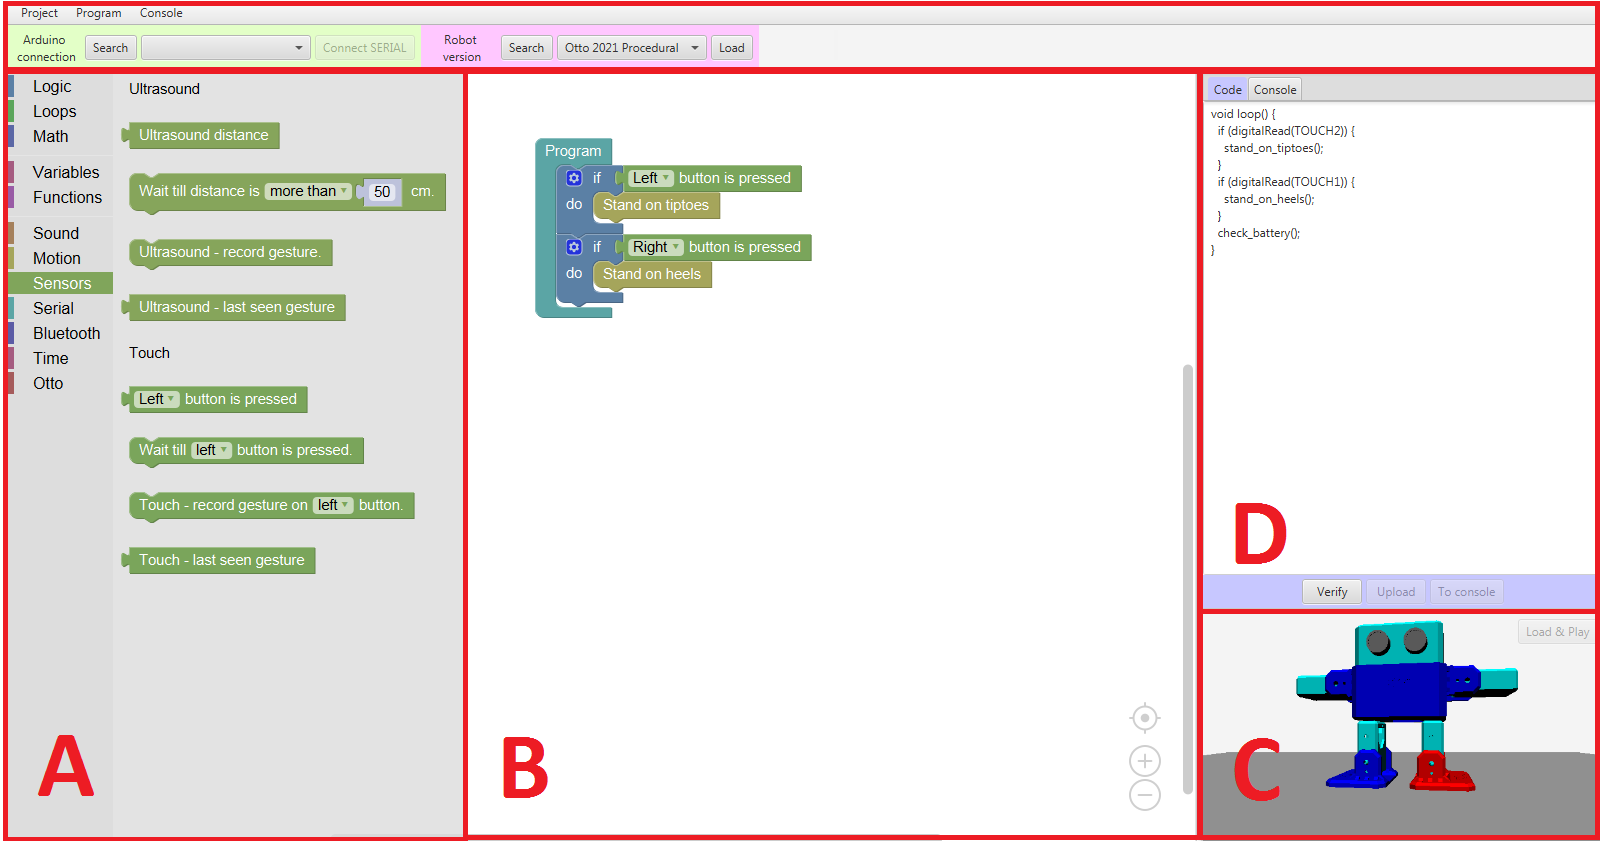
\includegraphics[width=1\textwidth]{images/rozlozenie-gui}}
\caption[Rozloženie používateľského rozhrania]{Rozloženie používateľského rozhrania}
\label{obr:gui-layout}
\end{figure}


% Editor kódu
\section{Editor kódu}
aka blokové paradigmy, odporúčania tvorcov, uvedomiť si kto je publikum, šetriť s počtom blokov, zobraziť len tie čo sa aktuálne dajú použiť

\subsection{Obrazový programovací jazyk}
- granularita puzzle
- pre rozne vekove kategorie (na zaklade poziadaviek)
- premenne - problem s typmi


% Vizualizacia
\section{Vizualizácia}
Implementáciu modulu vizualizácie začíname integráciou grafického prvku zobrazujúceho výstup simulácie v používateľskom rozhraní našej aplikácie. Herný charakter použitej technológie jMonkeyEngine (skr. jME, kapitola \ref{sub:herny-program}) umožňuje jednoduché vytvorenie aplikácie --- hry, ktorej jediné grafické okno pozostáva z výstupu simulácie. V našom prípade je ale simulácia len \uv{doplnkom}, rozhodli sme sa ju preto integrovať do hlavného okna našej aplikácie vo vymedzenom priestore, ako vidno na obrázku \ref{obr:gui-layout}. K tomuto účelu je nám nápomocné riešenie \textit{JME3--JFX} \cite{jmejfx}, ktoré umožňuje vykresľovanie grafického výstupu simulácie v jME priamo do komponentu \textit{ImageView} JavaFX scény. Samotná integrácia je potom už len jednoduchým volaním metódy prepájajúcej inštanciu jME s inštanciou ImageView.

V ďalšom je potrebné vyskladať model robota Otto a samotnú scénu --- prostredie, v ktorom sa bude simulovaný model pohybovať. Pre účely jednoduchej simulácie scénu v základe tvorí rovná plocha. V jazyku jME to znamená vytvorenie jedného širokého hlbokého nízkeho kvádra a jeho umiestnenie do stredu scény. Hornú stenu vzniknutej \uv{podlahy} možno vidieť na obrázkoch \ref{obr:otto-without-collision} a \ref{obr:otto-with-collision} pod modelom robota.

\subsection{Model robota Otto}
todo, tinkerpad, 3d tlac - existujuce modely
- 1.pokus: zobrazenie fixne, rotacia jednotlivych casti
- problemy s fyzikou, komplexita mesh collision shape -> riesenie je boxCollisionShape
- jonts = servo?
- obrazky - motor 130 deg.

OTTO
 - animacia = moyna len prednahrata, pred nas nepouzitelne
 - nodes .. create pivot points of rotation (1. pokus)
 - 2.pokus = pivot points reprezentovane hinges a riadenie hinge SW
 - BulletAppState = objekt pre interakciu s intergoovanzm jBullet
- register to physisc space ˇ(of te bullappstste)
reg. do phy. = tvar a mass
bulletAppState.setDebugEnabled(true);
use setPhysicsLocation() instead of setLocalTranslation() now, since you are dealing with a physical object.
geometria dostane control!
dynamic PhysicsControl, you can use setLinearVelocity() and apply forces and torques to it
animacia = vztvorenie modelu, bones, nasledna deformacia mesh v yavislosti od poyicie kosti, Jme = len predpripravene animacie


\subsection{Kamera --- }
camera movement




\begin{figure}
\centerline{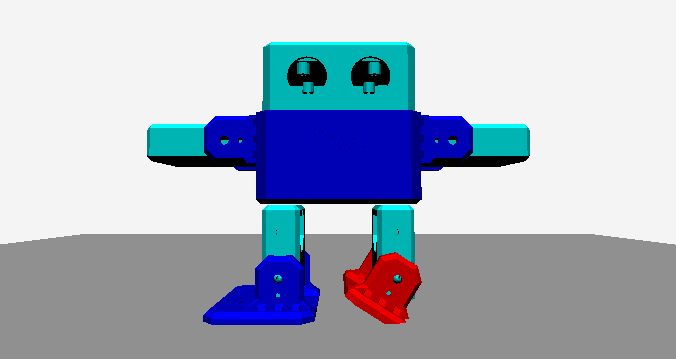
\includegraphics[width=0.4\textwidth]{images/otto-without-collision}}
\caption[Robot Otto - simulácia bez detekcie kolízií]{Robot Otto - simulácia bez detekcie kolízií}
\label{obr:otto-without-collision}
\end{figure}

\begin{figure}
\centerline{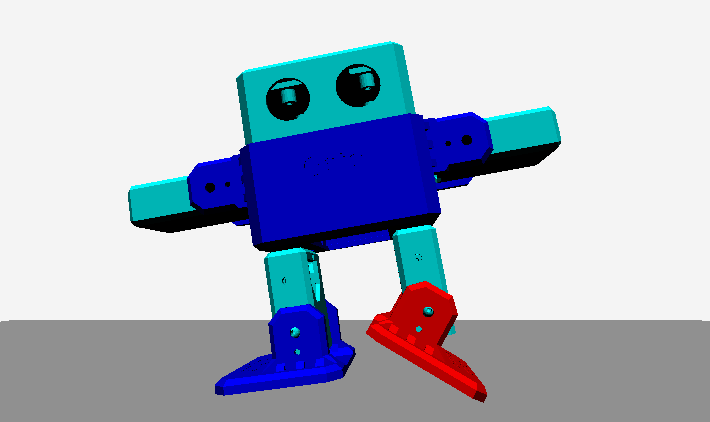
\includegraphics[width=0.4\textwidth]{images/otto-with-collision}}
\caption[Robot Otto - simulácia s detekciou kolízií]{Robot Otto - simulácia s detekciou kolízií}
\label{obr:otto-with-collision}
\end{figure}


% Komunikacia
\section{Komunikácia s robotom}
Možnosť komunikácie s robotom je jednou zo základných požiadaviek na našu aplikáciu. Umožňuje vyššiu interakciu s používateľom a je tiež nápomocná pri ladení programov (pomocné výpisy). Komunikácia s robotom na úrovni nahratia kompilovaného programu je predmetom časti \ref{sub:arduinoIDE}, tu je opísaná sériová komunikácia už bežiaceho programu v mikropočítači Arduino s našou aplikáciou. Jedná sa o komplementárnu časť systému k časti implementovanej v mikropočítači (sekcia \ref{sub:arduino}).

\subsubsection{Komunikácia zo strany aplikácie}
V aplikácii je cieľom vytvoriť integrovaný terminál pre sériovú komunikáciu. Mikropočítač Arduino komunikuje po pripojení rozhraním USB a nainštalovaní príslušného ovládača v počítači s OS, ktorý nám toto spojenie sprostredkuje. Podobne pracuje i terminál v Arduino IDE (oficiálne IDE pre vývoj riadiacich programov Arduino) alebo program Putty (klient pre ssh, Telnet, Rlogin a sériovú komunikáciu \cite{putty}). Autori mikropočítača odporúčajú pre implementáciu sériovej komunikácie v Java použitie knižníc \cite{arduinoAndJava}. V článku o prepojení Java --- Arduino sú spomínané dve, údajne nespoľahlivá knižnica RXTX a možná alternatíva, knižnica jSerialComm, ktorú použijeme. 

jSerialComm je platformovo nezávislá knižnica, ľahko integrovateľná do našej aplikácie \cite{jSerialComm}. Umožňuje vyhľadávať pripojené dostupné sérové porty, ako aj obojsmernú komunikáciu po pripojení. Podporuje niekoľko typov operácie, v závislosti na blokovaní čítania z (zápisu do) sériového portu. V prípade čítania sú na výber alternatívy ako \textit{neblokovaná komunikácia}, v ktorej možno príkazom \textit{read()} skúsiť načítať dáta, ak však nie sú k dispozícii (neboli prijaté), vrátený je prázdny reťazec. Inou možnosťou je vynútenie čakania na možný príchod správy a to buď len po nejaký čas alebo až do jej prijatia. Vo všetkých týchto prípadoch by ale v našej aplikácii bolo nutné cyklicky kontrolovať, či nejaké dáta nie sú k dispozícii (ako v mikropočítači), knižnica ale poskytuje vhodnejší prístup, registráciu callback funkcie. Tú knižnica zavolá po každom výskyte špecifikovanej udalosti, ktorom môže byť dostupnosť dát alebo prijatie ucelenej správy. V implementácii volíme možnosť volania callback funkcie po prijatí ucelenej správy, pričom za koniec správy je považovaný znak konca riadku (\textbackslash n --- line feed). Registrovaná callback funkcia správu načíta a zobrazí v termináli používateľovi.

Odosielanie správ je rovnako možné nastaviť do blokujúceho režimu, kde pri pokuse o zápis do sériového portu knižnica čaká buď to určitý čas alebo kým sa podarí odoslať požadovaný počet bajtov. Pre implementáciu volíme neblokovaný prístup, ak používateľ odošle dáta, sú zapísané hneď ako je to možné. Neblokovaný prístup umožní odoslanie viacerých správ, ktoré následne v rovnakom poradí knižnica odvysiela.


% Kompilácia a upload
\section{Kompilácia a nahranie riadiaceho programu}
\label{sub:arduinoIDE}
Kompiláciu a nahranie riadiaceho programu pri vývoji programov pre Arduino zvyčajne zabezpečuje Arduino IDE s grafickým používateľským rozhraním (sekcia \ref{sub:arduino}). Nahrávanie kompilovaného programu prebieha sériovou komunikáciou medzi Arduino IDE a bootloader programom v mikropočítači, zodpovednom za uloženie prijatého kódu do flash pamäte \cite{sketchUpload}. Overenie prenosu je uskutočnené spätným odoslaním celého programu z mikropočítača do IDE. Bootloader je spustený len určitý (krátky) čas po resetovaní procesora, ak v tomto časovom okne nie je zaznamenané nahrávanie riadiaceho programu, spustí sa posledný nahraný program. Procesor je resetovaný po obnove napájania ale i pri nadviazaní nového sériového spojenia.

Proces kompilácie a nahratia riadiaceho programu je možné implementovať na nižšej úrovni, samostatným volaním kompilátora a následného použitia knižnice jSerialComm pre jeho nahratie a spätnú verifikáciu. Pre kompiláciu je v tomto prípade možné použiť napríklad \textit{Arduino builder} \cite{arduinoBuilder}. Nástroj už ale nie je vývojármi udržiavaný, odporúčanou alternatívou je \textit{Arduino CLI}, poskytujúci robustnejšie riešenie. Umožňuje kompiláciu a zároveň i nahratie riadiaceho programu do mikropočítača. Problémom tohto riešenia je naopak aktívny vývoj, autori upozorňujú na možné zásadné zmeny do vydania verzie 1.0.0 \cite{arduinoCli}.

Implementovaným riešením je použitie CLI samotného Arduino IDE, ktoré poskytuje všetky nami požadované funkcionality \cite{arduinoIdeCli}. Vyskladaním riadiaceho programu v grafickom jazyku je vytvorený súbor, vstup pre Arduino IDE, ktoré je v Java spustené ako samostatný proces na pozadí. Prostredníctvom CLI je do Arduino IDE odovzdaný vyskladaný riadiaci program a parametre sériového portu, cez ktorý prebehne nahranie. Požadovaný sériový port zvolí používateľ v GUI našej aplikácie pomocou knižnice jSerialComm. Textový výstup procesu bežiaceho na pozadí je presmerovaný do grafického prvku aplikácie, kde je možné sledovať výsledky či prípadné chyby. Arduino IDE je tiež možné použiť bez pripojenia sériového portu na overenie vytvoreného programu.


% Riadiaci program robota
\section{Riadiaci program robota}
todo

\subsection{Robot Otto}
todo














